\section{Мета-обучение}

\subsection*{Классификация}

Набор данных отображаем в объект мета-признакового пространства.

Набор алгоритмов отображаем в оценки его качества на датасете
и ставим в соответствие мета-объекту лучший алгоритм.

Получаем набор данных для мета-классификации, на котором можно
обучить новый алгоритм и решить задачу выбора алгоритма для
конкретного набора данных по метапризнакам.

\subsection*{Регрессия}

Вместо предсказания метки можно предсказывать ошибку алгоритма и
получить задачу регрессии ошибки.

Значение функции качества можно нормализовать, но не по алгоритмам
а по наборам данных, т.к. важно относительное качество на одном
датасете.

\subsection*{Мягкая классификация}

Можно сводить к задаче мягкой классификации (задаче
предсказания распределения вероятностей). Для преобразования
оценок качества в вероятности можно использовать SoftArgMax:

$p_i = \frac{exp(Q_i / t)}{\sum_j exp(Q_j / t)}$,
где $t$ температура.

В качестве функции потерь можно использовать
\begin{itemize}
    \item $CrossEntropy(p, \hat{p}) = \sum p_i \log (\hat{p_i})$
    \item $KL(p, \hat{p}) = \sum p_i, \log(\frac{\hat{p_i}}{p_i})$
\end{itemize}

\subsection*{Ранжирование}

Для выбора алгоритма важно относительное качество, то есть можно
решать ранжирование. Но тут предполагается, что лидеры могут быть
отдельно протестированы, иначе зачем мы решали ранжирование.

Можно строить рексистемы для выбора алгоритма.

Типы рексистем:
\begin{itemize}
    \item Один алгоритм
    \item Неупорядоченное подмножество алгоритмов
    \item Полное линейное ранжирование
    \item Полное квазилинейное ранжирование
    (на доверительных интервалах)
    \item Неполное квазилинейное ранжирование
\end{itemize}

\begin{figure}[H]
    \centering
    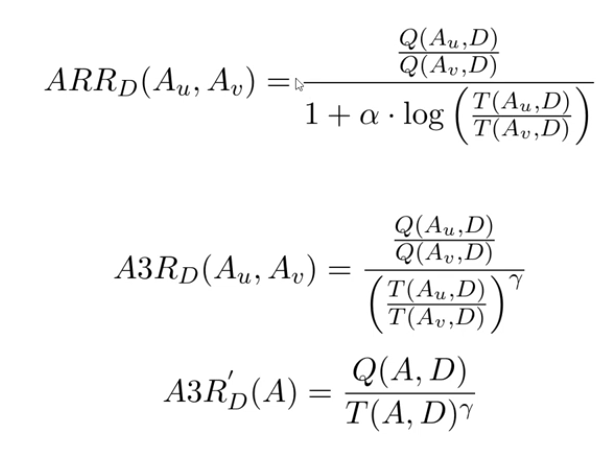
\includegraphics[scale=.4]{images/qvstime}
    \caption{В качестве оценки можно комбинировать
    функцию качества и оценку времени работы}
\end{figure}

\subsection*{Выбор гиперпараметров}

Мета-обучение можно применять для подбора гиперпараметров.
Для построения мета-набора данных для каждого алгоритма необходимо
необходимо запустить процесс настройки гиперпараметров. Появится
необходимость предсказания множества величин, и качество может
упасть. Вместо этого можно для пары из датасета и конфигурации
гиперпараметров предсказывать качество работы алгоритма.
